% This is a self-contained tex taken from USENIX style latex template. 
\documentclass[letter,twocolumn,10pt]{article}
\usepackage[margin=1in]{geometry}
\usepackage{enumitem}
\usepackage{url}
\usepackage{makecell}
\usepackage{csquotes}
\usepackage{booktabs}
\usepackage{tabularx}
\usepackage{tikz}
\usepackage{amsmath}
\usepackage{graphicx}
\usepackage{subfig}
\usepackage{float}
\usepackage{caption}
%\usepackage{subcaption}
\usepackage[numbers,sort&compress]{natbib}
\usepackage[super]{nth}
\usepackage{breakurl}
\usepackage[breaklinks]{hyperref}
\def\UrlBreaks{\do\/\do-}

\setlength{\textheight}{9.0in}
\setlength{\columnsep}{0.33in}
\setlength{\textwidth}{7.00in}
\setlength{\topmargin}{0.0in}
\setlength{\headheight}{0.0in}
\setlength{\headsep}{0.0in}
\addtolength{\oddsidemargin}{-0.25in}
\addtolength{\evensidemargin}{-0.25in}

\def\@maketitle{\newpage
 \vbox to 2.5in{
 \vspace*{\fill}
 \vskip 2em
 \begin{center}%
  {\Large\bf \@title \par}%
  \vskip 0.375in minus 0.300in
  {\large\it
   \lineskip .5em
   \begin{tabular}[t]{c}\@author
   \end{tabular}\par}%
 \end{center}%
 \par
 \vspace*{\fill}
 }
}

\usepackage{listings}
\usepackage{xcolor}
\definecolor{codegreen}{rgb}{0,0.6,0}
\definecolor{codegray}{rgb}{0.5,0.5,0.5}
\definecolor{codepurple}{rgb}{0.58,0,0.82}
\definecolor{backcolour}{rgb}{0.95,0.95,0.92}
\lstdefinestyle{mystyle}{
    backgroundcolor=\color{backcolour},   
    commentstyle=\color{codegreen},
    keywordstyle=\color{magenta},
    numberstyle=\tiny\color{codegray},
    stringstyle=\color{codepurple},
    basicstyle=\ttfamily\footnotesize,
    breakatwhitespace=false,         
    breaklines=true,                 
    captionpos=b,                    
    keepspaces=true,                 
    numbers=left,                    
    numbersep=5pt,                  
    showspaces=false,                
    showstringspaces=false,
    showtabs=false,                  
    tabsize=2
}
\lstset{style=mystyle}

\begin{filecontents}{\jobname.bib}
@Book{arpaciDusseau18:osbook,
  author =       {Arpaci-Dusseau, Remzi H. and Arpaci-Dusseau Andrea C.},
  title =        {Operating Systems: Three Easy Pieces},
  publisher =    {Arpaci-Dusseau Books, LLC},
  year =         2015,
  edition =      {1.00},
  note =         {\url{http://pages.cs.wisc.edu/~remzi/OSTEP/}}
}
@InProceedings{waldspurger02,
  author =       {Waldspurger, Carl A.},
  title =        {Memory resource management in {VMware ESX} server},
  booktitle =    {USENIX Symposium on Operating System Design and
                  Implementation (OSDI)},
  year =         2002,
  pages =        {181--194},
  note =         {\url{https://www.usenix.org/legacy/event/osdi02/tech/waldspurger/waldspurger.pdf}}
}
@inproceedings{CooperSTRS10socc,
  author    = {Brian F. Cooper and
               Adam Silberstein and
               Erwin Tam and
               Raghu Ramakrishnan and
               Russell Sears},
  title     = {Benchmarking cloud serving systems with {YCSB}},
  booktitle = {Proceedings of the 1st {ACM} Symposium on Cloud Computing, SoCC 2010,
               Indianapolis, Indiana, USA, June 10-11, 2010},
  pages     = {143--154},
  year      = {2010},
  doi       = {10.1145/1807128.1807152}
}
@misc{leveldb,
    author={Google},
    title={LevelDB},
    howpublished={\url{https://github.com/google/leveldb}}
}
@misc{rocksdb,
    author={Facebook},
    title={RocksDB},
    howpublished={\url{https://github.com/facebook/rocksdb}}
}
@inproceedings{usenixsilk,
author = {Oana Balmau and Florin Dinu and Willy Zwaenepoel and Karan Gupta and Ravishankar Chandhiramoorthi and Diego Didona},
title = {{SILK}: Preventing Latency Spikes in Log-Structured Merge Key-Value Stores},
booktitle = {2019 {USENIX} Annual Technical Conference ({USENIX} {ATC} 19)},
year = {2019},
isbn = {978-1-939133-03-8},
address = {Renton, WA},
pages = {753--766},
url = {https://www.usenix.org/conference/atc19/presentation/balmau},
publisher = {{USENIX} Association},
month = jul,
}

\end{filecontents}

\begin{document}

\date{}

%-------------------------------------------------------------------------------
%TODO You should come up with a compelling title. 
\title{\Large \textbf{Experience of Implementing SILK in LevelDB}}
%TODO Your name. 
\author{Kai Li, Qi Zhang and Yili Luo}
%-------------------------------------------------------------------------------
\maketitle

%-------------------------------------------------------------------------------
\section*{Abstract}
%-------------------------------------------------------------------------------
Log-Structured-Merge (LSM) key-value store is known to be effective and effcient when processing write-intensive workloads. Existing implementations of LSM key-value stores (e.g., LevelDB, RocksDB) have been widely used and adopted. However, current implementations of LSM incur high tail latency due to the inteference between clients' operations and LSM internal operations, namely the compactions. SILK is a novel technique proposed to solve this problem by cordinating these two kinds of operations. The idea is to throttle the IO bandwidth that can be used by the compaction threads on higher levels during the peak of clients' operations. The prototype of SILK is imelmented as an extension on RocksDB. In this project, we aim to implement the novel technique proposed by SILK in LevelDB. During our implementation, we identified several challenges and proposed an alternative solution based on the essence distilled from SILK, our alternative solution LevelDBSILK demonstrated promising performance improvement when handling write workloads. Currently, our solution performed poorly when handling read-intensive workloads, future work is proposed to improve the read performance.
%-------------------------------------------------------------------------------
\section{Introduction}
%-------------------------------------------------------------------------------
Log-Structured-Merge (LSM) tree is designed to improve the performance when processing write-intensive workloads. The most two popular implementations of LSM key-value store are LevelDB ~\cite{leveldb} and RocksDB ~\cite{rocksdb}. However, a recent research paper SILK ~\cite{usenixsilk} has shown the current design of LSM incurs high tail latency when handling write-intensive workloads. The root cause of such tail latency is the interference between clients' operations (reads/writes) and LSM internal operations (e.g., compactions). Due to lack of coordination between clients' opetations and internal operations, the compactions may use up the system's IO bandwidth and block the flushing work of memtable and evetually lead to a full memtable which blocks the clients' write operations. To mitigate the tail latency, SILK proposed a novel technology which prioritizes the compactions at the lower levels and limits the IO bandwidth that can be used by compactions at higher levels. The essence of SILK is to minimize the possibility of level 0 becomes full, therefore the memtable can be always flushed to level 0.

The prototype of SILK is implemented based on RocksDB. In this project, we aim to implement the same idea of SILK in LevelDB. However, after examing LevelDB's source code, we identified several challenges. First, unlike RocksDB which adopts multiple threads to do compactions, LevelDB merely adopts a single thread to do compaction. Second, SILK implements two thread queues to schedule those multiple compaction threads and prioritizes the threads at lower levels, we need to implement such two thread queues in LevelDB. Finally, SILK implements a client load minitor which guides SILK to throttle the IO bandwidth used by compaction threads at higher levels.

Given a short period time for this project, it is difficult to achieve the same level of implemtation as SILK in LevelDB. Instead, we choose to implement the essence of SILK which is to minimize the chance that level 0 becomes full during the peak of clients' opetations. To this end, we noticed that there are 2 Hyperparameters in LevelDB which control the size of level 0, we proposed to dynamically tune these Hyperparameters and control the size of level 0. Our proposed solution \textbf{LevelDBSILK} works by increasing the Hyperparameters during peak of clients' operations and decreasing it during the low load peroid. We implemented LevelDBSILK and conducted experiments by runing different workloads specified in \textsf{db\_bench}. The evaluation results show that compared with the native LevelDB, LevelDBSILK improves the write performance by $3X$.

The remainder of this report are orginized as follows. In section ~\ref{sec:preliminary}, we introduce the preliminaries of our project. Section ~\ref{sec:implementaion} elaborates on our implementation of SILK in LevelDB. Section ~\ref{sec:evaluation} evaluates the LevelDBSILK and compares it with LevelDB. Section ~\ref{sec:discussion} discuss our current implementaion of LevelDBSILK with future work listed in Section ~\ref{sec:futurework}. Section ~\ref{sec:conclusion} concludes the report.
%-------------------------------------------------------------------------------
\section{Preliminaries}
\label{sec:preliminary}
This section provides some preliminaries of this project.

\subsection {SILK's Design}
\label{sec:ioscheduler}
The prototype of SILK is implemented as an extension on RocksDB. SILK proposed a novel IO scheduler which aims to reduce interference between client operations and internal operations. The IO scheduler works as follows.
\begin{enumerate}
\item Opportunistically allocating more bandwidth to internal operations during periods of low load.
\item Implementing two thread queues, one for compaction threads at lower levels and the other one for higher levels. It prioritizes compaction threads at the lower levels.
\item Allowing compaction threads at lower levels to preempt that at higher levels, in order to facilitate the compaction work at lower levels.
\end{enumerate}

%\subsection {LevelDB's Compaction}
%\label{sec:leveldbcom}
%To implement SILK in LevelDB, the first step is to understand how LevelDB conducts the compaction work. LevelDB adopts two levels of compactions, namely minor compaction and major compaction. Figure ~\ref{leveldb_comaction} shows the Function Call Graph (FCG) of compaction in LevelDB. We elaborate on these two compactions as follows.
%
%\begin{figure*}[!htbp]
%\centering
%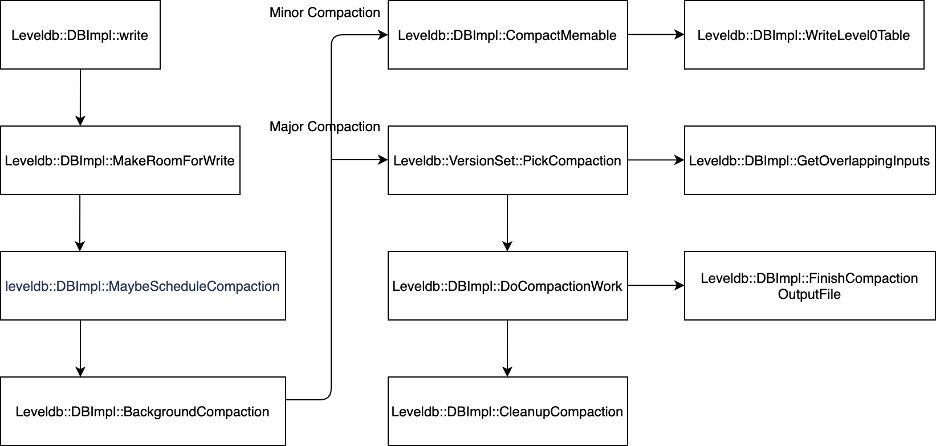
\includegraphics[width=0.8\textwidth]{./leveldb_comaction.png}
%\caption{Compaction Function Call Graph in LevelDB}
%\label{leveldb_comaction}
%\end{figure*}
%

LevelDB adopts a single thread to do compaction. Once a write operation starts, it will call the \textit{Write} function, inside \textit{Write}, \textit{MakeRoomForWrite} will be triggered. \textit{MakeRoomForWrite} implements a write control mechanism using two Hyperparameters: \textit{kL0\_SlowdownWritesTrigger} (8 by default) and \textit{kL0\_StopWritesTrigger} (12 by default). If the number of files at level 0 reaches to \textit{kL0\_SlowdownWritesTrigger}, LevelDB will slow down each write operation by 1ms. If the number of file reaches to \textit{kL0\_StopWritesTrigge}, all writes will be blocked. 

\textit{MaybeScheduleCompaction} is the entry of the actual compaction work. Three conditions can trigger this function to be executed.
\begin{enumerate}
\item \textit{manual\_compaction\_ != NULL}, user triggers the compaction manually.
\item \textit{imm\_ != NULL}, the Memtable is not NULL pointer and needs to be dumped to SSTable. This refers to the minor compaction.
\item \textit{versions\_$-$$>$NeedsCompaction}, some level needs compaction according to the compaction score. This refers to the major compaction.
\end{enumerate}

Then the thread will continue to invoke \textit{BacgroundCompaction} and start minor compaction and major compaction based on the above conditions.
For a minor compaction, it will be triggered as long as the following two conditions hold simutaneously: 1) memtable exceeds 4MB (defined by \textit{options\_.write\_buffer\_size}); 2) \textit{immutable == NULL}, the Memtable will be rotated to an immutable Memtable first which is further dumped to an SSTable and inserted to the disk.
 
For a major compaction, it will be triggered by one of following four conditions: 1) Manual trigger; 2) \textit{allowed\_seek} used up, every file has a seek limitation, once a seek miss happens, this number will be decreased by one and once it s used up, the compaction will start; 3) The numner of files at level 0 exceeds \textit{kL0\_CompactionTrigger} (4 by default); 4) Size at level i (i$>$0) exceeds $10^i$ MB.
%-------------------------------------------------------------------------------
\section{Implementation}
\label{sec:implementaion}
This section illustrates the challenges we encountered when implementing SILK in LevelDB. We proposed an alternative way to implement the core idea of SILK in LevelDB instead of duplicating the same level implementation of SILK.
 
\subsection {Challenges}
As discussed in Section ~\ref{sec:ioscheduler}, SILK's IO scheduler is implemented as an extension on RocksDB which schedules multiple compaction threads with different priority. However, when implementing the same idea in LevelDB, an inherent limitation is LevelDB only allows single thread to do compaction.We summarize the challenges of implementing SILK in LevelDB as follows.   
\begin{enumerate}
\item The first challenge is to implement a multiple threads based compaction in LevelDB.
\item The second challenge is to implement two thread queues with different priority when conducting compaction work.
\item The third challenge is to implement a client load monitor and throttle the IO bandwidth that can be used by the compaction threads.
\end{enumerate}

\subsection {Alternative Implementation - LevelDBSILK}
Given the time constraint of three weeks, we believe it is difficult to achieve the same level of implementation of SILK. The intuition of SILK is to minimize the possibility that flushing work is blocked by a full level $0$ in LSM. In other words, the main purpose of SILK is to minimize the chance that LSM has a full level $0$ when processing write-intensive workloads. With the same intuition in mind, we identified an alternative solution called \textbf{LevelDBSILK} that achieves the purpose similar to SILK. Recall in \ref{sec:leveldbcom}, LevelDB adopts two Hyperparameters to control the compaction at level $0$. \textit{kL0\_SlowdownWritesTrigger} is the threshold of slowing down each write operation by 1 ms, \textit{kL0\_StopWritesTrigger} is the threshold of blocking a write operation until the compaction work is finished at level $0$. LevelDBSILK achieves the purpose similar to SILK by dynamically tuning these Hyperparameters. At a high level, during peak of client operations, LevelDBSILK increases these Hyperparameters whenever the current value is hitted by the number of files at level $0$. And during the low load peroid of client operations, LevelDBSILK decreases the Hyperparameters until it drop to the initial value.

\lstinputlisting[label=lst:code, language=C++, caption=Source Code of LevelDBSILK]{LevelDBSILK.cpp}
Listing ~\ref{lst:code} shows the code snippet of Hyperparameters increasing part in LevelDBSILK. In line $10$ and $28$, we double the Hyperparameter once it is hitted. We defer the Hyperparameters decreasing part to future work.
%-------------------------------------------------------------------------------
\section{Evaluation}
\label{sec:evaluation}
%-------------------------------------------------------------------------------
\subsection {Experimental Environment}
In this project, we conducted experiments on a machine equipped with Intel 4-core
i5-7500 CPU of 3.40 GHz with 8 MB cache, a 8 GB RAM and 256 GB disk. We ran the workloads speficied in \textsf{db\_bench}. 

\subsection {Reproduce the Problem in LevelDB}
\label{sec:reproduce}

The root cause of high tail latency comes from the fact that level 0 is full when handling write-intensive workloads in a short peroid of time. A full level 0 blocks the flush of memtable and eventually leads to a full memtable. In order to reproduce a full level $0$, we noticed that in \textsf{db\_bench}, there are two options which can be configured to reproduce the desired case, namely \textit{value\_size} and \textit{write\_buffer\_size}. For instance, set a large \textit{value\_size} along with a small \textit{write\_buffer\_size} can fill up the memtable quickly, therefore, flushing happens frequently and can lead to a full level $0$ in a short period of time. To this end, we set \textit{value\_size} to $30$ KB and \textit{write\_buffer\_size} to $64$ KB, which means every 3 write operations can fill up the memtable. We choose a pure-write workload \textbf{fillsync} and drive 1000 operations (through option \textit{num}) to reporduce the high tail latency problem.

The experiment result is presented in Figure ~\ref{db_bench}. It can be seen that the amortized latency is $23.359$ ms/op and throughput is $1.2$ MB/s. Since we did not capture the latency of each write operation, the output does not show how many times the latency spike occurs. However, we can estimate it by counting the occurrence of `slow down' (line $9$) and `blocking' (line $26$) in the log. From the log, we count $607$ occurrences of `slow down' and $164$ occurrences of `blocking'.  

\begin{figure}[H]
\centering
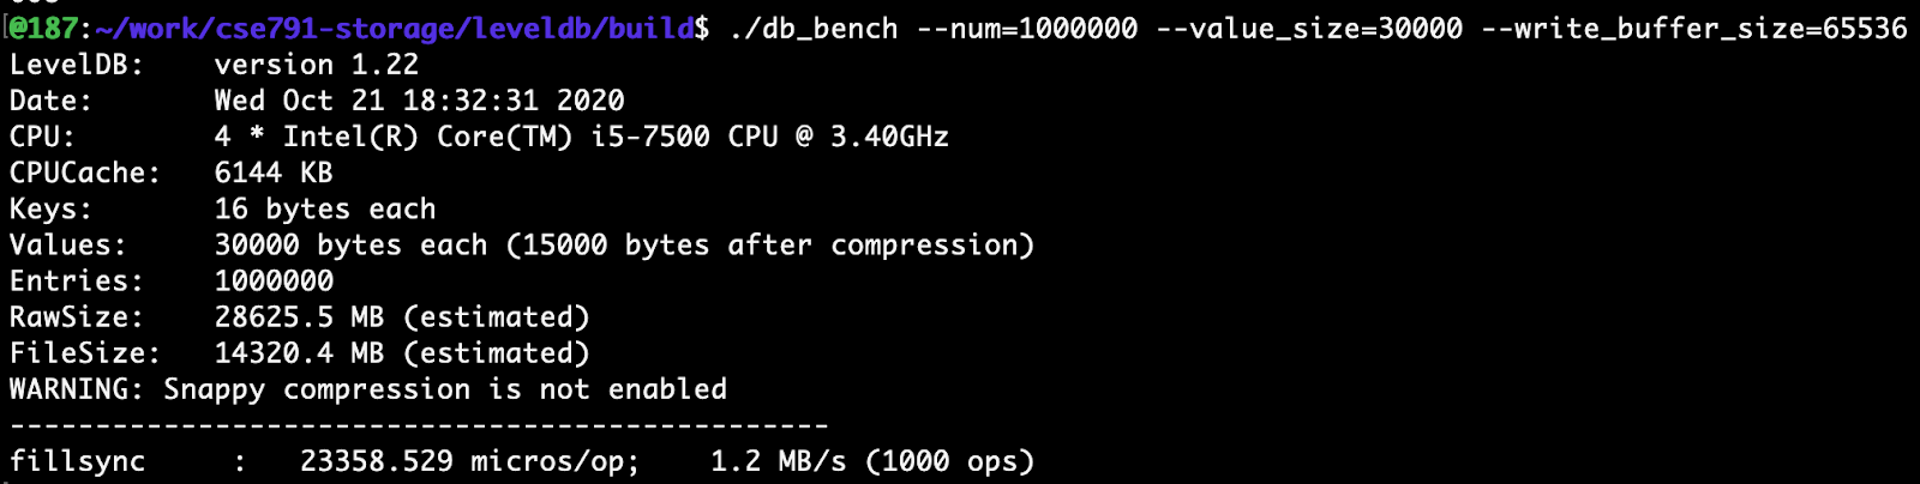
\includegraphics[width=0.5\textwidth]{./db_bench_leveldb.png}
\caption{Run fillsync in LevelDB}
\label{db_bench}
\end{figure}

\subsection {Run LevelDBSILK}
Under the same setting as described in ~\ref{sec:reproduce}, we test LevelDBSILK with the same workload. The experiment result is presented in Figure ~\ref{db_bench_1}. It can be seen that the amortized latency is $7.802$ ms/op and throughput is $3.7$ MB/s. From the log, we count $6$ occurrences of `slow down' and $6$ occurrences of `blocking'. The experiment result shows LevelDBSILK reduces the latency by $3X$ compared with native LevelDB when processing a pure-write workload.  

\begin{figure}[H]
\centering
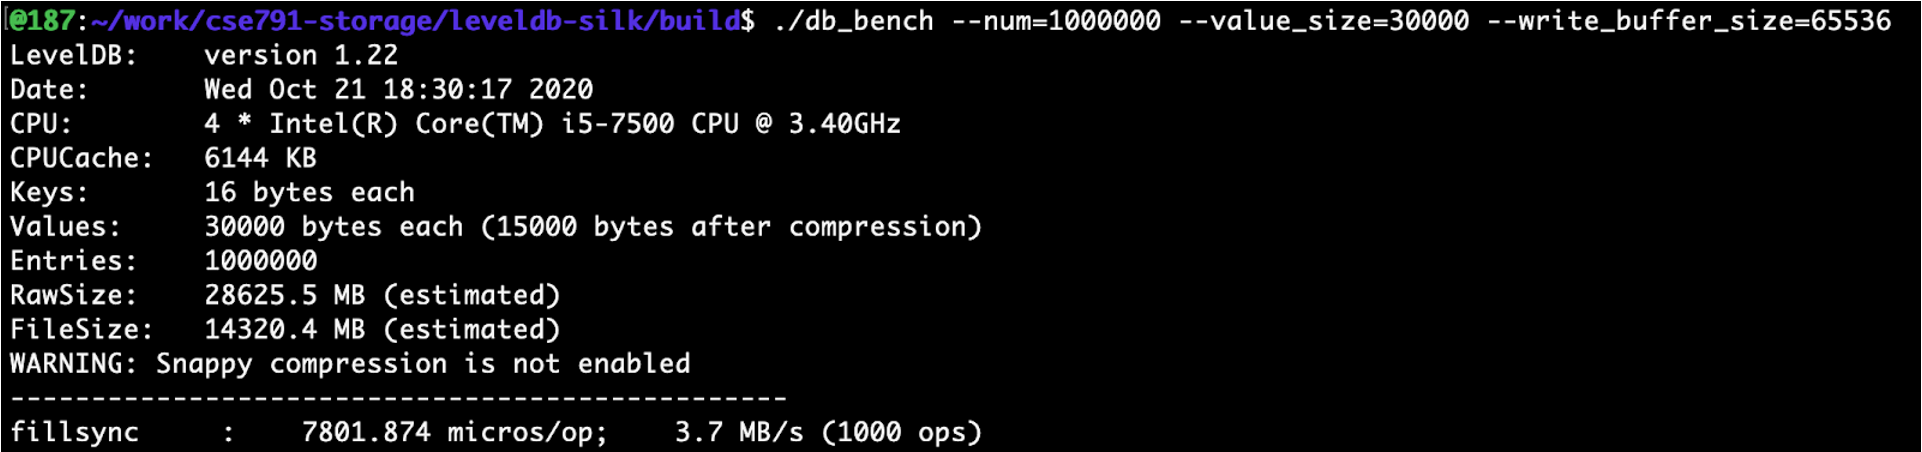
\includegraphics[width=0.5\textwidth]{./db_bench_leveldbsilk.png}
\caption{Run fillsync in LevelDBSILK}
\label{db_bench_1}
\end{figure}

\subsection {Run Multiple Workloads}
Under the same setting as described in ~\ref{sec:reproduce}, we run all the workloads specified in \textsf{db\_bench}, including read-intensive workloads and write-intensive workloads and compare the performance of LevelDB and LevelDBSILK. The experiment results are summarized in table ~\ref{comparison}.

\begin{table}
	\centering 
	\footnotesize
	\begin{tabular}{c|l|c}
		\hline
		\bf{{Workloads}} & \bf{{LevelDB}}  & \bf{{LevelDBSILK}} \\ \hline
		fillseq & \makecell{5.880 ms} & 5.619 ms \\ \hline 
		fillsync & \makecell{9.332 ms} & 8.293 ms \\ \hline
		fillrandom & \makecell{22.076 ms} & 4.501 ms \\ \hline
		overwrite & \makecell{37.279 ms} & 4.628 ms \\ \hline
		readrandom & \makecell{4.769 us} & 54.319 us \\ \hline
		readseq & \makecell{1.310 us} & 10.603 us \\ \hline
		readreverse & \makecell{4.132 us} & 16.178 us \\ \hline
	\end{tabular}
	\caption{Performance comparison of LevelDB and LevelDBSILK}
	\label{comparison}
\end{table}

From the table, it can be found that for pure-write workloads, including \textit{fillseq, fillsync, fillrandom, overwrite}, LevelDBSILK achieves better performance than LevelDB. For pure-read workloads such as \textit{readrandom, readseq, readreverse}, LevelDBSILK achieves worse performance than LevelDB. LevelDBSILK achieves worse read performance due to the larger level 0, because we haven't implemented the Hyperparameters decreasing part and after running those pure-write workloads, LevelDBSILK produces a large number of files at level 0 before executing those pure-read workloads.  

%-------------------------------------------------------------------------------
\section{Discussion}
\label{sec:discussion}
Currently, LevelDBSILK increases the Hyperparameters everytime when the current value is hitted and there is no upper limit on these Hyperparameters. One may concern that these Hyperparameters may increase indefinitely. To prevent it from growing indefinitely, one can add an upper limit to cap these Hyperparameters and the implementation should be simple. However, we believe these Hyperparameters should not grow to a huge number, if this situation happens, it implies that the workloads contain a long-run of write-intensive opetaions and the size of Memtable grows faster than level 0. In this case, even SILK cannot mitigate the tail latency problem.    
%-------------------------------------------------------------------------------

\section{Future Work}
\label{sec:futurework}
For the future work, we plan to implement a client requests monitor as the guidence to dynamically tune the Hyperparameters in order to achieve better performance. Other than the client requests monitor, we will implement the Hyperparameters decreasing part to improve the read performance. 

\section{Conclusion}
\label{sec:conclusion}
In this report, we share the experience of implementing SILK in LevelDB. During the implementation, we identified several challenges due to the inherent difference between RocksDB and LevelDB. Instead of achieving the same level implementaion, we proposed an alternative solution to achieve the purpose similar to SILK. Our proposed solution works by dynamically tuning the Hyperparameters that control the size of level $0$ in LevelDB. The evaluation results show that our solution achieves $3X$ improvement than the native LevelDB when processing write-intensive workloads.  

{\footnotesize 
\bibliographystyle{acm}
\bibliography{p2}
}
\end{document}
